% Created by tikzDevice version 0.12.3.1 on 2023-04-12 14:24:24
% !TEX encoding = UTF-8 Unicode
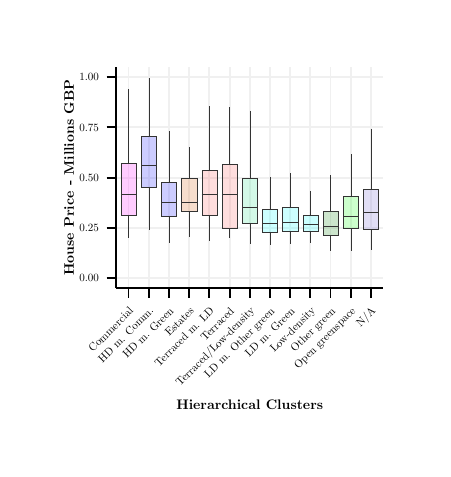
\begin{tikzpicture}[x=1pt,y=1pt]
\definecolor{fillColor}{RGB}{255,255,255}
\path[use as bounding box,fill=fillColor,fill opacity=0.00] (0,0) rectangle (142.64,152.15);
\begin{scope}
\path[clip] (  0.00,  0.00) rectangle (142.64,152.15);
\definecolor{fillColor}{RGB}{255,255,255}

\path[fill=fillColor] (  0.00,  0.00) rectangle (142.64,152.15);
\end{scope}
\begin{scope}
\path[clip] ( 32.06, 58.04) rectangle (128.41,137.92);
\definecolor{fillColor}{RGB}{255,255,255}

\path[fill=fillColor] ( 32.06, 58.04) rectangle (128.41,137.92);
\definecolor{drawColor}{gray}{0.94}

\path[draw=drawColor,line width= 0.7pt,line join=round] ( 32.06, 61.67) --
	(128.41, 61.67);

\path[draw=drawColor,line width= 0.7pt,line join=round] ( 32.06, 79.82) --
	(128.41, 79.82);

\path[draw=drawColor,line width= 0.7pt,line join=round] ( 32.06, 97.98) --
	(128.41, 97.98);

\path[draw=drawColor,line width= 0.7pt,line join=round] ( 32.06,116.13) --
	(128.41,116.13);

\path[draw=drawColor,line width= 0.7pt,line join=round] ( 32.06,134.29) --
	(128.41,134.29);

\path[draw=drawColor,line width= 0.7pt,line join=round] ( 36.44, 58.04) --
	( 36.44,137.92);

\path[draw=drawColor,line width= 0.7pt,line join=round] ( 43.74, 58.04) --
	( 43.74,137.92);

\path[draw=drawColor,line width= 0.7pt,line join=round] ( 51.04, 58.04) --
	( 51.04,137.92);

\path[draw=drawColor,line width= 0.7pt,line join=round] ( 58.34, 58.04) --
	( 58.34,137.92);

\path[draw=drawColor,line width= 0.7pt,line join=round] ( 65.64, 58.04) --
	( 65.64,137.92);

\path[draw=drawColor,line width= 0.7pt,line join=round] ( 72.94, 58.04) --
	( 72.94,137.92);

\path[draw=drawColor,line width= 0.7pt,line join=round] ( 80.23, 58.04) --
	( 80.23,137.92);

\path[draw=drawColor,line width= 0.7pt,line join=round] ( 87.53, 58.04) --
	( 87.53,137.92);

\path[draw=drawColor,line width= 0.7pt,line join=round] ( 94.83, 58.04) --
	( 94.83,137.92);

\path[draw=drawColor,line width= 0.7pt,line join=round] (102.13, 58.04) --
	(102.13,137.92);

\path[draw=drawColor,line width= 0.7pt,line join=round] (109.43, 58.04) --
	(109.43,137.92);

\path[draw=drawColor,line width= 0.7pt,line join=round] (116.73, 58.04) --
	(116.73,137.92);

\path[draw=drawColor,line width= 0.7pt,line join=round] (124.03, 58.04) --
	(124.03,137.92);
\definecolor{drawColor}{gray}{0.20}

\path[draw=drawColor,line width= 0.1pt,line join=round] ( 43.74,113.00) -- ( 43.74,134.07);

\path[draw=drawColor,line width= 0.1pt,line join=round] ( 43.74, 94.65) -- ( 43.74, 79.05);
\definecolor{fillColor}{RGB}{0,0,255}

\path[draw=drawColor,line width= 0.1pt,fill=fillColor,fill opacity=0.20] ( 41.00,113.00) --
	( 41.00, 94.65) --
	( 46.47, 94.65) --
	( 46.47,113.00) --
	( 41.00,113.00) --
	cycle;

\path[draw=drawColor,line width= 0.1pt] ( 41.00,102.32) -- ( 46.47,102.32);

\path[draw=drawColor,line width= 0.1pt,line join=round] ( 36.44,103.32) -- ( 36.44,129.97);

\path[draw=drawColor,line width= 0.1pt,line join=round] ( 36.44, 84.55) -- ( 36.44, 76.26);
\definecolor{fillColor}{RGB}{255,0,255}

\path[draw=drawColor,line width= 0.1pt,fill=fillColor,fill opacity=0.20] ( 33.70,103.32) --
	( 33.70, 84.55) --
	( 39.18, 84.55) --
	( 39.18,103.32) --
	( 33.70,103.32) --
	cycle;

\path[draw=drawColor,line width= 0.1pt] ( 33.70, 91.86) -- ( 39.18, 91.86);

\path[draw=drawColor,line width= 0.1pt,line join=round] ( 87.53, 86.40) -- ( 87.53, 98.33);

\path[draw=drawColor,line width= 0.1pt,line join=round] ( 87.53, 78.33) -- ( 87.53, 73.60);
\definecolor{fillColor}{RGB}{0,255,255}

\path[draw=drawColor,line width= 0.1pt,fill=fillColor,fill opacity=0.20] ( 84.80, 86.40) --
	( 84.80, 78.33) --
	( 90.27, 78.33) --
	( 90.27, 86.40) --
	( 84.80, 86.40) --
	cycle;

\path[draw=drawColor,line width= 0.1pt] ( 84.80, 81.45) -- ( 90.27, 81.45);

\path[draw=drawColor,line width= 0.1pt,line join=round] ( 94.83, 87.19) -- ( 94.83, 99.76);

\path[draw=drawColor,line width= 0.1pt,line join=round] ( 94.83, 78.52) -- ( 94.83, 73.83);

\path[draw=drawColor,line width= 0.1pt,fill=fillColor,fill opacity=0.20] ( 92.10, 87.19) --
	( 92.10, 78.52) --
	( 97.57, 78.52) --
	( 97.57, 87.19) --
	( 92.10, 87.19) --
	cycle;

\path[draw=drawColor,line width= 0.1pt] ( 92.10, 81.90) -- ( 97.57, 81.90);

\path[draw=drawColor,line width= 0.1pt,line join=round] (109.43, 85.91) -- (109.43, 98.90);

\path[draw=drawColor,line width= 0.1pt,line join=round] (109.43, 77.02) -- (109.43, 71.47);
\definecolor{fillColor}{RGB}{0,128,0}

\path[draw=drawColor,line width= 0.1pt,fill=fillColor,fill opacity=0.20] (106.70, 85.91) --
	(106.70, 77.02) --
	(112.17, 77.02) --
	(112.17, 85.91) --
	(106.70, 85.91) --
	cycle;

\path[draw=drawColor,line width= 0.1pt] (106.70, 80.33) -- (112.17, 80.33);

\path[draw=drawColor,line width= 0.1pt,line join=round] ( 65.64,100.51) -- ( 65.64,123.69);

\path[draw=drawColor,line width= 0.1pt,line join=round] ( 65.64, 84.23) -- ( 65.64, 75.16);
\definecolor{fillColor}{RGB}{255,85,85}

\path[draw=drawColor,line width= 0.1pt,fill=fillColor,fill opacity=0.20] ( 62.90,100.51) --
	( 62.90, 84.23) --
	( 68.37, 84.23) --
	( 68.37,100.51) --
	( 62.90,100.51) --
	cycle;

\path[draw=drawColor,line width= 0.1pt] ( 62.90, 91.91) -- ( 68.37, 91.91);

\path[draw=drawColor,line width= 0.1pt,line join=round] ( 51.04, 96.29) -- ( 51.04,114.72);

\path[draw=drawColor,line width= 0.1pt,line join=round] ( 51.04, 83.87) -- ( 51.04, 74.44);
\definecolor{fillColor}{RGB}{0,0,255}

\path[draw=drawColor,line width= 0.1pt,fill=fillColor,fill opacity=0.20] ( 48.30, 96.29) --
	( 48.30, 83.87) --
	( 53.77, 83.87) --
	( 53.77, 96.29) --
	( 48.30, 96.29) --
	cycle;

\path[draw=drawColor,line width= 0.1pt] ( 48.30, 89.11) -- ( 53.77, 89.11);

\path[draw=drawColor,line width= 0.1pt,line join=round] ( 72.94,102.73) -- ( 72.94,123.65);

\path[draw=drawColor,line width= 0.1pt,line join=round] ( 72.94, 79.60) -- ( 72.94, 76.32);
\definecolor{fillColor}{RGB}{255,85,85}

\path[draw=drawColor,line width= 0.1pt,fill=fillColor,fill opacity=0.20] ( 70.20,102.73) --
	( 70.20, 79.60) --
	( 75.67, 79.60) --
	( 75.67,102.73) --
	( 70.20,102.73) --
	cycle;

\path[draw=drawColor,line width= 0.1pt] ( 70.20, 91.83) -- ( 75.67, 91.83);

\path[draw=drawColor,line width= 0.1pt,line join=round] (102.13, 84.35) -- (102.13, 92.98);

\path[draw=drawColor,line width= 0.1pt,line join=round] (102.13, 78.55) -- (102.13, 74.34);
\definecolor{fillColor}{RGB}{0,255,255}

\path[draw=drawColor,line width= 0.1pt,fill=fillColor,fill opacity=0.20] ( 99.40, 84.35) --
	( 99.40, 78.55) --
	(104.87, 78.55) --
	(104.87, 84.35) --
	( 99.40, 84.35) --
	cycle;

\path[draw=drawColor,line width= 0.1pt] ( 99.40, 81.07) -- (104.87, 81.07);

\path[draw=drawColor,line width= 0.1pt,line join=round] ( 80.23, 97.82) -- ( 80.23,122.18);

\path[draw=drawColor,line width= 0.1pt,line join=round] ( 80.23, 81.35) -- ( 80.23, 73.80);
\definecolor{fillColor}{RGB}{37,229,137}

\path[draw=drawColor,line width= 0.1pt,fill=fillColor,fill opacity=0.20] ( 77.50, 97.82) --
	( 77.50, 81.35) --
	( 82.97, 81.35) --
	( 82.97, 97.82) --
	( 77.50, 97.82) --
	cycle;

\path[draw=drawColor,line width= 0.1pt] ( 77.50, 87.25) -- ( 82.97, 87.25);

\path[draw=drawColor,line width= 0.1pt,line join=round] (116.73, 91.31) -- (116.73,106.49);

\path[draw=drawColor,line width= 0.1pt,line join=round] (116.73, 79.62) -- (116.73, 71.36);
\definecolor{fillColor}{RGB}{0,255,0}

\path[draw=drawColor,line width= 0.1pt,fill=fillColor,fill opacity=0.20] (114.00, 91.31) --
	(114.00, 79.62) --
	(119.47, 79.62) --
	(119.47, 91.31) --
	(114.00, 91.31) --
	cycle;

\path[draw=drawColor,line width= 0.1pt] (114.00, 84.20) -- (119.47, 84.20);

\path[draw=drawColor,line width= 0.1pt,line join=round] ( 58.34, 97.69) -- ( 58.34,108.95);

\path[draw=drawColor,line width= 0.1pt,line join=round] ( 58.34, 85.82) -- ( 58.34, 76.38);
\definecolor{fillColor}{RGB}{212,85,0}

\path[draw=drawColor,line width= 0.1pt,fill=fillColor,fill opacity=0.20] ( 55.60, 97.69) --
	( 55.60, 85.82) --
	( 61.07, 85.82) --
	( 61.07, 97.69) --
	( 55.60, 97.69) --
	cycle;

\path[draw=drawColor,line width= 0.1pt] ( 55.60, 89.21) -- ( 61.07, 89.21);

\path[draw=drawColor,line width= 0.1pt,line join=round] (124.03, 93.81) -- (124.03,115.67);

\path[draw=drawColor,line width= 0.1pt,line join=round] (124.03, 79.19) -- (124.03, 71.79);
\definecolor{fillColor}{RGB}{106,90,205}

\path[draw=drawColor,line width= 0.1pt,fill=fillColor,fill opacity=0.20] (121.29, 93.81) --
	(121.29, 79.19) --
	(126.77, 79.19) --
	(126.77, 93.81) --
	(121.29, 93.81) --
	cycle;

\path[draw=drawColor,line width= 0.1pt] (121.29, 85.40) -- (126.77, 85.40);

\path[] ( 32.06, 58.04) rectangle (128.41,137.92);
\end{scope}
\begin{scope}
\path[clip] (  0.00,  0.00) rectangle (142.64,152.15);
\definecolor{drawColor}{RGB}{0,0,0}

\path[draw=drawColor,line width= 0.7pt,line join=round] ( 32.06, 58.04) --
	( 32.06,137.92);
\end{scope}
\begin{scope}
\path[clip] (  0.00,  0.00) rectangle (142.64,152.15);
\definecolor{drawColor}{RGB}{0,0,0}

\node[text=drawColor,anchor=base east,inner sep=0pt, outer sep=0pt, scale=  0.40] at ( 25.76, 60.29) {0.00};

\node[text=drawColor,anchor=base east,inner sep=0pt, outer sep=0pt, scale=  0.40] at ( 25.76, 78.45) {0.25};

\node[text=drawColor,anchor=base east,inner sep=0pt, outer sep=0pt, scale=  0.40] at ( 25.76, 96.60) {0.50};

\node[text=drawColor,anchor=base east,inner sep=0pt, outer sep=0pt, scale=  0.40] at ( 25.76,114.76) {0.75};

\node[text=drawColor,anchor=base east,inner sep=0pt, outer sep=0pt, scale=  0.40] at ( 25.76,132.91) {1.00};
\end{scope}
\begin{scope}
\path[clip] (  0.00,  0.00) rectangle (142.64,152.15);
\definecolor{drawColor}{RGB}{0,0,0}

\path[draw=drawColor,line width= 0.7pt,line join=round] ( 28.56, 61.67) --
	( 32.06, 61.67);

\path[draw=drawColor,line width= 0.7pt,line join=round] ( 28.56, 79.82) --
	( 32.06, 79.82);

\path[draw=drawColor,line width= 0.7pt,line join=round] ( 28.56, 97.98) --
	( 32.06, 97.98);

\path[draw=drawColor,line width= 0.7pt,line join=round] ( 28.56,116.13) --
	( 32.06,116.13);

\path[draw=drawColor,line width= 0.7pt,line join=round] ( 28.56,134.29) --
	( 32.06,134.29);
\end{scope}
\begin{scope}
\path[clip] (  0.00,  0.00) rectangle (142.64,152.15);
\definecolor{drawColor}{RGB}{0,0,0}

\path[draw=drawColor,line width= 0.7pt,line join=round] ( 32.06, 58.04) --
	(128.41, 58.04);
\end{scope}
\begin{scope}
\path[clip] (  0.00,  0.00) rectangle (142.64,152.15);
\definecolor{drawColor}{RGB}{0,0,0}

\path[draw=drawColor,line width= 0.7pt,line join=round] ( 36.44, 54.54) --
	( 36.44, 58.04);

\path[draw=drawColor,line width= 0.7pt,line join=round] ( 43.74, 54.54) --
	( 43.74, 58.04);

\path[draw=drawColor,line width= 0.7pt,line join=round] ( 51.04, 54.54) --
	( 51.04, 58.04);

\path[draw=drawColor,line width= 0.7pt,line join=round] ( 58.34, 54.54) --
	( 58.34, 58.04);

\path[draw=drawColor,line width= 0.7pt,line join=round] ( 65.64, 54.54) --
	( 65.64, 58.04);

\path[draw=drawColor,line width= 0.7pt,line join=round] ( 72.94, 54.54) --
	( 72.94, 58.04);

\path[draw=drawColor,line width= 0.7pt,line join=round] ( 80.23, 54.54) --
	( 80.23, 58.04);

\path[draw=drawColor,line width= 0.7pt,line join=round] ( 87.53, 54.54) --
	( 87.53, 58.04);

\path[draw=drawColor,line width= 0.7pt,line join=round] ( 94.83, 54.54) --
	( 94.83, 58.04);

\path[draw=drawColor,line width= 0.7pt,line join=round] (102.13, 54.54) --
	(102.13, 58.04);

\path[draw=drawColor,line width= 0.7pt,line join=round] (109.43, 54.54) --
	(109.43, 58.04);

\path[draw=drawColor,line width= 0.7pt,line join=round] (116.73, 54.54) --
	(116.73, 58.04);

\path[draw=drawColor,line width= 0.7pt,line join=round] (124.03, 54.54) --
	(124.03, 58.04);
\end{scope}
\begin{scope}
\path[clip] (  0.00,  0.00) rectangle (142.64,152.15);
\definecolor{drawColor}{RGB}{0,0,0}

\node[text=drawColor,rotate= 45.00,anchor=base east,inner sep=0pt, outer sep=0pt, scale=  0.40] at ( 38.37, 49.51) {Commercial};

\node[text=drawColor,rotate= 45.00,anchor=base east,inner sep=0pt, outer sep=0pt, scale=  0.40] at ( 45.67, 49.51) {HD m. Comm.};

\node[text=drawColor,rotate= 45.00,anchor=base east,inner sep=0pt, outer sep=0pt, scale=  0.40] at ( 52.97, 49.51) {HD m. Green};

\node[text=drawColor,rotate= 45.00,anchor=base east,inner sep=0pt, outer sep=0pt, scale=  0.40] at ( 60.26, 49.51) {Estates};

\node[text=drawColor,rotate= 45.00,anchor=base east,inner sep=0pt, outer sep=0pt, scale=  0.40] at ( 67.56, 49.51) {Terraced m. LD};

\node[text=drawColor,rotate= 45.00,anchor=base east,inner sep=0pt, outer sep=0pt, scale=  0.40] at ( 74.86, 49.51) {Terraced};

\node[text=drawColor,rotate= 45.00,anchor=base east,inner sep=0pt, outer sep=0pt, scale=  0.40] at ( 82.16, 49.51) {Terraced/Low-density};

\node[text=drawColor,rotate= 45.00,anchor=base east,inner sep=0pt, outer sep=0pt, scale=  0.40] at ( 89.46, 49.51) {LD m. Other green};

\node[text=drawColor,rotate= 45.00,anchor=base east,inner sep=0pt, outer sep=0pt, scale=  0.40] at ( 96.76, 49.51) {LD m. Green};

\node[text=drawColor,rotate= 45.00,anchor=base east,inner sep=0pt, outer sep=0pt, scale=  0.40] at (104.06, 49.51) {Low-density};

\node[text=drawColor,rotate= 45.00,anchor=base east,inner sep=0pt, outer sep=0pt, scale=  0.40] at (111.36, 49.51) {Other green};

\node[text=drawColor,rotate= 45.00,anchor=base east,inner sep=0pt, outer sep=0pt, scale=  0.40] at (118.66, 49.51) {Open greenspace};

\node[text=drawColor,rotate= 45.00,anchor=base east,inner sep=0pt, outer sep=0pt, scale=  0.40] at (125.96, 49.51) {N/A};
\end{scope}
\begin{scope}
\path[clip] (  0.00,  0.00) rectangle (142.64,152.15);
\definecolor{drawColor}{RGB}{0,0,0}

\node[text=drawColor,anchor=base,inner sep=0pt, outer sep=0pt, scale=  0.50] at ( 80.23, 14.03) {\bfseries Hierarchical Clusters};
\end{scope}
\begin{scope}
\path[clip] (  0.00,  0.00) rectangle (142.64,152.15);
\definecolor{drawColor}{RGB}{0,0,0}

\node[text=drawColor,rotate= 90.00,anchor=base,inner sep=0pt, outer sep=0pt, scale=  0.50] at ( 16.70, 97.98) {\bfseries House Price - Millions GBP};
\end{scope}
\end{tikzpicture}
